% This document is based on the RSC LaTeX template, but extensively modified,
% https://www.rsc.org/journals-books-databases/journal-authors-reviewers/author-tools-services/
% most importantly we are using LuaLaTeX instead of pdflatex in order to compile 
% our large TiKZ/PGF plots (pdflatex cannot handle large memory requirements)

\documentclass[9pt,twoside,twocolumn]{article}\usepackage{knitr}

% ----------------------------------------------------------------------
% Page layout
% ----------------------------------------------------------------------
\usepackage{extsizes}
\usepackage{balance}
\usepackage[left=1.5cm,right=1.5cm,top=1.785cm,bottom=2.0cm]{geometry}
% ----------------------------------------------------------------------


% ----------------------------------------------------------------------
% Bibliography
% ----------------------------------------------------------------------
\usepackage[backend=biber,doi=true,style=chem-rsc]{biblatex}
\addbibresource{references/library.bib}
% modification: make DOI string a hyperlink in the list of references
\newcommand*\doiformat[1]{\small#1}
\DeclareFieldFormat{doi}{%
   \mkbibacro{\small{DOI}}\addcolon\space
   \ifhyperref{\href{https://dx.doi.org/#1}{\doiformat{#1}}}{\doiformat{#1}}%
}
% ----------------------------------------------------------------------


% ----------------------------------------------------------------------
% Fonts and symbols
% ----------------------------------------------------------------------
% \usepackage{luatextra} % also loads fixltx2e, fontspec, xunicode
\usepackage[utf8]{luainputenc}
% DO NOT use package xunicode with luatex: gives errors with tikzDevice/knitr
% https://tex.stackexchange.com/questions/401481/charter-font-shape-undefined-with-lualatex/401658
\usepackage{fontspec}
\setmainfont{XCharter}
\setromanfont{XCharter}
\setsansfont{Liberation Sans}
\setmonofont{Liberation Mono}
\usepackage{textcomp} % \textdegree, \textmu, \texttrademark and some other symbols
% ----------------------------------------------------------------------


% ----------------------------------------------------------------------
% Support packages - general
% ----------------------------------------------------------------------
\usepackage[english]{babel}
% % modification: gitinfo2 used to help keep track of manuscript versions
% \usepackage{gitinfo2}
\usepackage[compact]{titlesec}
\usepackage{sectsty}
\usepackage{fancyhdr}
\usepackage{csquotes}
\usepackage{setspace} % setstretch{} used later in the preamble
% ----------------------------------------------------------------------


% ----------------------------------------------------------------------
% Support packages - graphics, captions, footnotes, etc.
% ----------------------------------------------------------------------
\usepackage{graphicx}
\usepackage[%
   format=plain,
   justification=justified,
   singlelinecheck=false,
   font={stretch=1.125,small,sf},
   labelfont=bf,
   labelsep=space]{caption}
\usepackage{subcaption}
\usepackage{tikz}
% RSC template calls for float pkg, but I cannot detect that it's used
%\usepackage{float}
\usepackage{fnpos} % controls the positions of footnotes
\definecolor{cream}{RGB}{222,217,201} % RSC colour: cream
% ----------------------------------------------------------------------


% ----------------------------------------------------------------------
% Support packages - tables, lists
% ----------------------------------------------------------------------
\usepackage{booktabs}
\usepackage[inline]{enumitem}
% Reset table and figure numbering in SI (S1, S2 and so on)
% https://www.stat.berkeley.edu/~paciorek/computingTips/Customizing_numbering_pages.html
% http://bytesizebio.net/2013/03/11/adding-supplementary-tables-and-figures-in-latex/
\newcommand{\startsupplement}{%
   \setcounter{table}{0}%
   \renewcommand{\thetable}{S\arabic{table}}%
   \setcounter{figure}{0}%
   \renewcommand{\thefigure}{S\arabic{figure}}%
}
% ----------------------------------------------------------------------


% ----------------------------------------------------------------------
% Support packages - chemistry, science
% ----------------------------------------------------------------------
\usepackage{amssymb}
\usepackage{chemformula}
   \setchemformula{charge-style=math}
\usepackage{siunitx}
\sisetup{%
   uncertainty-mode=compact,%
   reset-text-family=false,%
   text-family-to-math=true,%
   range-phrase=\ensuremath{\text{ to }}%
}
   %https://tex.stackexchange.com/questions/56051/problem-with-options-in-declaresiunit
   \DeclareSIUnit[per-mode=symbol]{\molar}{\mole\per\cubic\deci\metre}
   \DeclareSIUnit[per-mode=symbol]{\micromolar}{\micro\mole\per\cubic\deci\metre}
   \DeclareSIUnit{\Molar}{\textsc{m}}
   \DeclareSIUnit{\vsNHE}{vs~NHE}
   \DeclareSIUnit{\voltNHE}{\volt\vsNHE}
\usepackage{chemfig}
   % setatomsep has been deprecated, use \setchemfig instead
   \setchemfig{atom sep=2em}
   % define invisible bond (for use between the charged species)
   \definesubmol\nobond{-[,1.2,,,draw=none]}
% ----------------------------------------------------------------------


% ----------------------------------------------------------------------
% Packages that need to be called last: hyperref, cleveref etc.
% ----------------------------------------------------------------------
% do not use [pagebackref]{hyperref}, not stable, gives errors
\usepackage{hyperref}
% modication: cleveref is indispensable
\usepackage[nameinlink]{cleveref}
% ----------------------------------------------------------------------


% ----------------------------------------------------------------------
% R SETUP
% ----------------------------------------------------------------------

% ----------------------------------------------------------------------


% ----------------------------------------------------------------------
% R LOAD PACKAGES
% ----------------------------------------------------------------------



% ----------------------------------------------------------------------




% !Rnw root = paper.Rnw






% !Rnw root = paper.Rnw



\IfFileExists{upquote.sty}{\usepackage{upquote}}{}
\begin{document}


\pagestyle{fancy}
\thispagestyle{plain}
\fancypagestyle{plain}{
   % Simple header without header graphics
   \renewcommand{\headrulewidth}{0pt}
}

\makeFNbottom
\makeatletter
   \renewcommand\LARGE{\@setfontsize\LARGE{15pt}{17}}
   \renewcommand\Large{\@setfontsize\Large{12pt}{14}}
   \renewcommand\large{\@setfontsize\large{10pt}{12}}
   \renewcommand\footnotesize{\@setfontsize\footnotesize{7pt}{10}}
\makeatother

\renewcommand{\thefootnote}{\fnsymbol{footnote}}
\renewcommand\footnoterule{\vspace*{1pt}% 
\color{cream}\hrule width 3.5in height 0.4pt \color{black}\vspace*{5pt}} 
\setcounter{secnumdepth}{5}

\makeatletter 
   \renewcommand\@makefntext[1]% 
   {\noindent\makebox[0pt][r]{\@thefnmark\,}#1}
\makeatother 
\renewcommand{\figurename}{\small{Fig.}~}
\sectionfont{\sffamily\Large}
\subsectionfont{\normalsize}
\subsubsectionfont{\bf}
\setstretch{1.125}
\setlength{\skip\footins}{0.8cm}
\setlength{\footnotesep}{0.25cm}
\setlength{\jot}{10pt}
\titlespacing*{\section}{0pt}{4pt}{4pt}
\titlespacing*{\subsection}{0pt}{15pt}{1pt}

\fancyfoot{}
% \fancyfoot[CO]{\vspace{-7.1pt}\hspace{13.2cm}}
% \fancyfoot[CE]{\vspace{-7.2pt}}
\fancyfoot[RO]{\footnotesize{\sffamily{\textbar \hspace{2pt}\thepage}}}
\fancyfoot[LE]{\footnotesize{\sffamily{\thepage~\textbar}}}
\fancyhead{}
\renewcommand{\headrulewidth}{0pt}
\renewcommand{\footrulewidth}{0pt}
\setlength{\arrayrulewidth}{1pt}
\setlength{\columnsep}{6.5mm}

\makeatletter 
   \newlength{\figrulesep} 
   \setlength{\figrulesep}{0.5\textfloatsep} 
   
   \newcommand{\topfigrule}{\vspace*{-1pt}% 
   \noindent{\color{cream}\rule[-\figrulesep]{\columnwidth}{1.5pt}} }

   \newcommand{\botfigrule}{\vspace*{-2pt}% 
   \noindent{\color{cream}\rule[\figrulesep]{\columnwidth}{1.5pt}} }

   \newcommand{\dblfigrule}{\vspace*{-1pt}% 
   \noindent{\color{cream}\rule[-\figrulesep]{\textwidth}{1.5pt}} }
\makeatother

\twocolumn[
  \begin{@twocolumnfalse}
   \vspace{3cm}
   \sffamily
   \begin{tabular}{m{4.5cm} p{13.5cm} }

   \textsf{\footnotesize DOI: 10.1021/acs.jpcc.9b11229} & 
      \noindent\LARGE{\textbf{Optical properties of ZnO quantum dots and effect of size on their photocatalytic activity$^\dag$}}\\
   \vspace{0.3cm} & \vspace{0.3cm}\\

   {\footnotesize\sffamily\textit{J.\ Phys.\ Chem.\ C} 2020, 124, 11} & 
      \noindent\large{Taha Ahmed\textit{$^{a}$} and Tomas Edvinsson\textit{$^{b\ddag}$}} \\

   \hspace{1.09in} & \noindent\normalsize{
      Zinc oxide is a well-known metal oxide and with its direct optical band gap, it
      provides a promising alternative to titanium oxide in photocatalytic applications.
      \ch{ZnO} is here studied as quantum dots (QDs) where ultra-small nanoparticles of
      \ch{ZnO} show optical quantum confinement with a band gap opening for particles below
      \qty{9}{\nm} in diameter from the shift of the band edge energies.
      The optical properties of growing \ch{ZnO} quantum dots are determined with
      Tauc-analysis and a system of QDs for treatment and degradation of distributed
      threats is analysed using an organic probe molecule, methylene blue.
      The effect of optical properties of the QDs and the kinetics of dye degradation
      are quantified for low-dimensional ZnO materials in the range of \qtyrange{3}{7}{\nm}
      and show a substantial increase in photocatalytic activity compared to larger
      \ch{ZnO} particles.
      This is attributed to a combined effect from the increased surface area as well
      as a quantum confinement effect that goes beyond the increased surface area.
      The results show a significantly higher photocatalytic activity for the QDs between
      \qtyrange[range-phrase=--]{3}{6}{\nm} with a complete decolouration of the model
      compound, while QDs from \qty{6}{\nm} and upwards in diameter show signs of competing
      reduction reactions.
      Our study demonstrates that ultra-small \ch{ZnO} particles have a reactivity beyond 
      that which is expected due to their increased surface area and also show
      size-dependent reaction pathways which introduces the possibility for a size
      selective catalysis.%
   }\\
   \end{tabular}
   \end{@twocolumnfalse} \vspace{0.6cm}
]


\rmfamily
\section*{}
\vspace{-1cm}


\footnotetext{\textit{$^{a}$~Department of Chemistry--{\AA}ngstr{\"o}m, Structural chemistry, Uppsala university.}}
\footnotetext{\textit{$^{b}$~Department of Engineering Sciences, Solid state physics, Uppsala university, Sweden; tomas.edvinsson@angstrom.uu.se}}

\footnotetext{%
   \dag~The published paper and its supplementary information is available online:\newline
   \url{https://pubs.acs.org/doi/full/10.1021/acs.jpcc.9b11229}%
}


% ----------------------------------------------------------------------
% Custom LaTeX commands
% ----------------------------------------------------------------------
% optical absorbance
\newcommand{\absorbance}{\ensuremath{A}}
% ----------------------------------------------------------------------



% references inside main paper (separated from refs in SI)
\begin{refsection}

% Code (data analysis)

% !Rnw root = paper.Rnw






































%%%%%%%%%%%%%%%%%%%%%%%%%%%%%%%%%%
%%% small NP
%%% NP initial size: SMALL
%%% NO STIRRING
























%%%%%%%%%%%%%%%%%%%%%%%%%%%%%%%%%%
%%% small NP
%%% NP initial size: SMALL
%%% NO STIRRING




















%%%%%%%%%%%%%%%%%%%%%%%%%%%%%%%%%%
%%% medium NP
%%% NP initial size: MEDIUM
%%% NO STIRRING
























%%%%%%%%%%%%%%%%%%%%%%%%%%%%%%%%%%
%%% large NP
%%% NP initial size: LARGE
%%% NO STIRRING





















%%%%%%%%%%%%%%%%%%%%%%%%%%%%%%%%%%
%%% large NP
%%% NP initial size: LARGE
%%% NO STIRRING





































































































% Body text

% !Rnw root = paper.Rnw


\section{Introduction}

Zinc oxide is an abundant and familiar material that has applications spanning from UV-absorbing additive in rubber \cite{Heideman2005} and sunscreens \cite{King2005,Serpone2007}, to high-tech applications in chemical sensing \cite{Rambu2013,Cai2013}, spintronics \cite{Sharma2004}, and photovoltaics \cite{Quintana2007,Boschloo2006}.
The wide interest in low-dimensional \ch{ZnO} for optoelectronic applications is fuelled by its high carrier mobility \cite{Yoshikawa1997,Look1998,Kaidashev2003}, its direct wide band gap ($E_\text{g}$ $\sim\qty{3.3}{\eV}$), and a large exciton binding energy of \qty{60}{\meV} \cite{Ozgur2005} allowing room-temperature exciton emission.
There are also intriguing size effects of \ch{ZnO} on the nano-scale below \qty{9}{\nm} in diameter, such as vibrational quantum confinement \cite{Raymand2012}, discontinuous exciton emission decay rate \cite{Jacobsson2014}, and quantum confined Stark effects \cite{Jacobsson2014a} that show that more is to be discovered even in this seemingly well-known material.
Here, we focus on the optical and photochemical properties of \ch{ZnO} quantum dots with a special focus towards their possible application as photocatalysts in colloidal suspension for the degradation of distributed environmental threats.

The formal quantum efficiency of photocatalysis is higher in smaller \ch{ZnO} quantum dots compared to larger ones and show an interplay between the accessible surface area and their ability to absorb photons in the solar spectrum \cite{Jacobsson2012} and is likely also related to the interaction and thus the weakening of excitons with charged surface states \cite{Jacobsson2014}.
Here it is interesting to compare the properties of wurtzite \ch{ZnO} with that of the more extensively studied anatase \ch{TiO2}.
Zinc oxide has a markedly higher absorption coefficient due to its direct band gap, almost the same conduction and valence band edges (\qty{-0.5}{\volt} and \qty{+2.8}{\voltNHE} at \mbox{pH\,5}) as \ch{TiO2} and the advantage of a higher charge carrier mobility \cite{Boschloo2006} showing more or less the same driving force for the reactions but a more effective absorption of light and improved carrier transport.
There are also several studies reporting a more effective photocatalytic degradation of organic dyes for ZnO compared to \ch{TiO2} \cite{Sakthivel2003,Muruganandham2006,Yan2009a}.
Although \ch{ZnO} does not have any intrinsic toxicology, the nanoscale size of the particles raises the issue of nano-toxicity where particles smaller than \qty{100}{\nm} typically introduce surface reactivities causing nanoscale toxicity \cite{Maynard2011, Maynard2011a}.
However, the higher reactivity for nanoscale materials is a desirable property for the degradation of environmental threats where the high surface areas and the ability to penetrate into porous materials, such as soot particles and oils, are advantageous.
If a dynamical nanoscale system, such as the slowly growing nanoparticles in this study, is applied towards photocatalysis the higher reactivity can be used when the particles are small and the system will then naturally be deactivated as the particles grow larger or aggregate among themselves or with their environment during the later stages of the process.
The system with the photoactive \ch{ZnO} shows slow system growth and coalescence into aggregates and natural sedimentation to the bottom of the contaminated water container or, if applied at larger scale, to the bottom of the pond or sea to become a part of the natural sediment, thus deactivating its nano-toxicity.
A key focus of our approach is to investigate the properties of low-dimensional \ch{ZnO} under growth by studying their optical and photocatalytic activity in the quantum confined regime ($d<\qty{9}{\nm}$) where the band gap of the particles changes during their growth with eventual aggregation and sedimentation for larger particles.

The United Nations World water development report \cite{WWAP2017} identifies the effective removal of emerging pollutants 
(such as pharmaceuticals, fragrances, pesticides and herbicides) 
as one of the main challenges for the European region of the world, and as a large concern in other regions, where environmental regulations and laws may still lag behind industrial practices.
When it comes to organic compounds, one effective approach to degrade such pollutants is to utilise the fact that the energy in UV-photons is high enough to break covalent bonds in molecules. 
For some unstable molecules such direct illumination is enough to degrade them, but generally a photocatalyst is needed to overcome the activation barriers and significantly improve the degradation kinetics. 
The effect is mediated \textit{via} various Reactive Oxygen Species (ROS), such as singlet oxygen \ch{^1O2}, superoxide radicals \ch{O2^{.-}},  hydroperoxyl radicals \ch{HO2^.}, hydroxyl radicals  \ch{^.OH}, and hydrogen peroxides \ch{H2O2} that are generated at the metal oxide surface upon UVA (\qtyrange{315}{400}{\nm}) irradiation in aqueous solutions \cite{Tachikawa2007}. 
For \ch{ZnO}, the photo-generated holes in the valence band are generated with a higher rate compared to the indirect band gap semiconductor \ch{TiO2}, while having the photogenerated hole still sufficiently low in energy and thus highly oxidising (see~\cref{fig:schematic-and-solarlamp}).
When water is present at the semiconductor surface, the photo-generated hole generates hydroxyl radicals (\ch{^.OH}) \cite{Herrmann2005,Chen2007d} that act as a strong non-selective oxidant. 
The end result is often a complete mineralisation of the undesired chemicals into \ch{CO2}, water and mineral acids.

In this paper, we show that a small change in \ch{ZnO} nanoparticle diameter leads to a large change in photocatalytic activity. The observed behaviour is a result of the size-dependent change of energy levels and the subsequent optical effect in the quantum-confined semiconductor system in aqueous suspension.





\section{Methods}

A series of methylene blue aqueous solutions of with concentrations of \qtylist{0.5;1;2;5;10;20;50;100}{\micromolar} were volumetrically prepared from methylene blue (powder, VWR Prolabo, CAS 61-73-4) weighed on a Mettler AT261 balance with \qty{0.01}{\mg} resolution, quantitatively transferred and diluted to the mark in volumetric glassware with deionised water (for volumes and dilution factors, see \cref{tabsi:mb-stock-solutions}). 
The dye solutions were stored in bluecap glass bottles wrapped in aluminium-foil and stored in the dark.

\ch{ZnO} nanoparticle suspensions were synthesised by mixing zinc acetate dihydrate, \ch{Zn(OAc)2 * 2 H2O}, Fluka, $\geqslant\qty{99.5}{\percent}$, and lithium hydroxide monohydrate, \ch{LiOH * H2O}, Sigma-Aldrich, $\geqslant\qty{99.0}{\percent}$, both dissolved in ethanol, \qty{99.5}{\percent}, following previously published routes \cite{Jacobsson2011,Meulenkamp1998,Spanhel1991}.
In brief, each precursor was dissolved in \ch{EtOH} and diluted to \qty{50}{\ml} (\textit{cf.} \cref{tabsi:precursor-solutions}). 
The precursor solutions were then quantitatively mixed and the time was noted (this represented the start of nanoparticle nucleation and growth).
Our modifications to previous work included heating the \ch{LiOH} solution to around \qty{45}{\celsius} while flushing the head space with \ch{N2} to both increase the solubility of lithium hydroxide and decrease the chance of formation of the carbonate. 
Just prior to mixing both precursor solutions were cooled in an ice bath for a few minutes.

In all PC experiments, one part of the \ch{ZnO(EtOH)} NP suspension was mixed with nine parts of \qty{10}{\micromolar} \ch{MB(aq)} directly into a \qty{10}{\mm} PMMA cuvette (typically $\qty{0.2}{\ml}+\qty{1.8}{\ml}$, so the cuvette contained \ch{H2O}:\ch{EtOH} 90:10 by volume), which after an initial thorough but fast mixing was with a solar simulator (\qty{100}{\mW\per\square\cm}, Oriel/Newport class~A solar simulator with an AM1.5G optical filter) while recording a full UV/Vis/NIR spectrum perpendicular to the direction of illumination each minute for the duration of the experiment.


The UV/Vis/NIR absorption measurements were performed using an OceanOptics HR-2000+ spectrometer with deuterium and halogen light sources.
In all our measurements, a spectrum with \num{2048} evenly distributed points from \qtyrange{190}{1100}{\nm} were sampled with an integration time of \qty{1}{\ms} (each saved spectrum averaged \num{10} such measurements) using fibre-optic cables from the lamp to the cuvette holder and back to the spectrometer, such that the face of the cuvette being illuminated by the solar lamp was unobstructed. 
We used PMMA cuvettes ($l=\qty{1}{\cm}$) with transparent walls and the top of the cuvette was left open to atmosphere during PC experiments. We observed some evaporative loss during a typical PC experiment (duration approximately \qty{150}{\minute}) but it was small and outweighed by the need to allow air into the cuvette.

Band gap analysis was performed using Tauc plots, where the square of the absorption was plotted as a function of photon energy. 
For a direct band gap semiconductor like \ch{ZnO}, the band gap is then given as the intercept of the fitted line with the abscissa. More details on the Tauc fit procedure can be found in the SI.

For all recorded spectra, the methylene blue absorption band (roughly \qtyrange{500}{800}{\nm}) was baseline-fitted with a cubic spline function and peak-fitted with two Gaussian kernels in an automatic fashion using the scripting-capabilities of Fityk~1.3.1 \cite{Wojdyr2010}. 
The baseline correction was needed because the baseline of the spectra increased continuously over the course of an experiment due to increased scattering, in turn due to processes involved with agglomeration of the nanoparticles with each other and with the organic species in solution over the course of an experiment.





\section{Results and discussion}

Under the scheme proposed in this paper, a suspension of \ch{ZnO} nanoparticles in their native growth solution would be added to a polluted water surface and with exposure to sunlight photocatalyse the breakdown of the organic pollutant followed by the aggregation and subsequent sedimentation of the catalyst particles themselves, effectively rendering them inert.
Here we spectrometrically track both the \ch{ZnO} band edge and the methylene blue (MB) absorption band \textit{in-situ} under simulated solar illumination to gain insights into both how the optical properties of the QDs change, the effect of growth upon dilution and their photocatalytic activity during the process.



\subsection{Optical properties of low-dimensional \ch{ZnO}}

\begin{figure}[tb]
\centering
\begin{subfigure}[b]{\linewidth}
\caption{}
\label{fig:schematic}
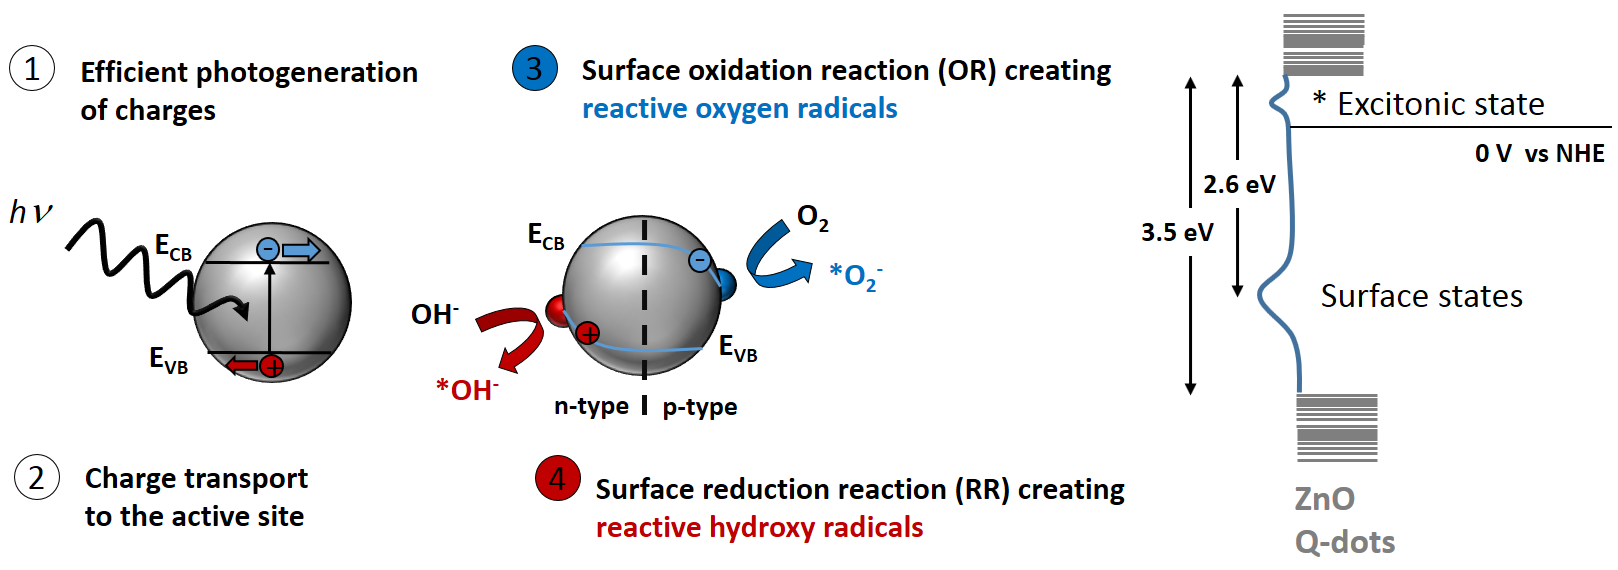
\includegraphics[width=\linewidth]{images/nanoparticle-redox}
\end{subfigure}\\%
\begin{subfigure}[b]{\linewidth}
\caption{}
\label{fig:solarlamp}
\begin{knitrout}\footnotesize
\definecolor{shadecolor}{rgb}{0.969, 0.969, 0.969}\color{fgcolor}

{\centering \includegraphics[width=3.40in]{figure/fig-solarlamp-1} 

}


\end{knitrout}
\end{subfigure}
\caption{(\subref{fig:schematic}) Schematic of the different processes occurring on a catalyst nanoparticle's surface during photocatalysis in water, along with an energy diagram of the electronic states in low-dimensional \ch{ZnO}.
(\subref{fig:solarlamp}) The ASTM AM1.5G solar spectrum (here shown only up to \qty{1000}{\nm}) overlaid with: UV absorbance of PMMA cuvette (grey area, \textit{c.f.} \cref{figsi:cuvette-PMMA-abs}), with the coloured areas showing the wavelength region of the solar spectrum absorbable by our smallest (yellow) and largest (blue) \ch{ZnO} NPs, respectively.
The areas shaded in darker yellow and darker blue underline part of the spectrum of our laboratory's AM1.5G solar simulator (which outputs less UV and more VIS than the ASTM reference).}
\label{fig:schematic-and-solarlamp}
\end{figure}


The optical properties of ultra-small \ch{ZnO} particles can theoretically be determined by solving the Schrödinger equation for the first excited state for a particle in a spherical well with radius $R$ for the kinetic energy and a higher frequency dielectric screening approach for the potential energy giving \cite{Brus1984,Jacobsson2011,Edvinsson2018}
\begin{equation}
E_\text{g} = %
E_\text{g,\,bulk} +
\frac{\hbar^{2}\pi^{2}}{2R^2} \left(\frac{1}{m_\text{e}^{*}} + \frac{1}{m_{h}^\text{*}}\right) %
- \frac{1.8e^2}{\varepsilon R} +
\frac{e^2}{R}\sum_{n=1}^{\infty} \alpha_\text{n} \left(\frac{r_\text{e} + r_\text{h}}{R}\right)^{2n}
\end{equation}
where $E_\text{g,bulk}$ is the band gap of the bulk material, $\hbar$ is Planck's constant, $\varepsilon$ is the dielectric constant of \ch{ZnO}, $e$ is the elementary charge, and $m_\text{e}^{*}$ and $m_\text{h}^{*}$ are the effective masses of the electron and hole, respectively.
The second term is the increased kinetic energy from the localisation of the electron-hole pair confined within a sphere with radius $R$ and scales as $R^{-2}$.
The third term is the Coloumb attraction in a screened environment and scales as $R^{-1}$.
The last term describes the average polarisability for an electron and hole at position $r_\text{e}$ and $r_\text{h}$, respectively, with a polarisability $\alpha_\text{n} = \frac{(\varepsilon_\text{rel} - 1)(n + 1)}{\varepsilon_2(\varepsilon_\text{n} + n + 1)}$ where $\varepsilon_\text{rel} = \frac{\varepsilon_2}{\varepsilon_1}$ is the relative dielectic constant of a material with $\varepsilon_2$ in an environment with the dielectric constant $\varepsilon_1$-.
This polarisation term goes to zero for a localised excitation in a screened environment, that is, if $r_\text{e} + r_\text{h} \ll R$. \cite{Brus1984}

This gives a physical justification for a functional dependence between the band gap, $E_\text{g}$, in \unit{\eV} and the particle diameter, $d$, in \unit{\nm} as $E_\text{g} = C_1 + \frac{C_2}{d} + \frac{C_3}{d^2}$ where the coefficients $C_n$ are to be found from experimental data. 
\textcite{Jacobsson2011} found that $C_1=\qty{3.301}{\eV}$, $C_2=\qty{0.293}{\eV\nm}$, and $C_3=\qty{3.94}{\eV\nm\squared}$ for low-dimensional \ch{ZnO} using growth conditions similar to ours.
One can note that the use of bulk band gap $E_\text{g}=\qty{3.301}{\eV}$ intrinsically includes the exciton absorption in \ch{ZnO} as this cannot be deconvoluted from the experimental absorption onset at room temperature. 
The mean diameter of the \ch{ZnO} nanoparticle ensemble is given by rearranging the previous formula into
\begin{equation}\label{eq:diameter}
d = \frac{2C_3}{-C_2 + \sqrt{C_2^2 - 4 C_3 (C_1 - E_\text{g})}}\text{.}
\end{equation}


To quantify the photocatalytic properties of the distributed particles, and in order to get a better idea of how the material would perform under natural sunlight, we used an AM1.5G solar simulator lamp (\textit{c.f.} \cref{fig:solarlamp}). \cite{ASTMG17303}
The large band gap of \ch{ZnO} severely restricts the number of solar photons the material can absorb, and this is further exacerbated initially by the large band gap of the smallest-diameter particles.
At $E\geqslant\qty{3.78}{\eV}$ only \qty{0.14}{\percent} of the AM1.5G photon flux is available to the \ch{ZnO} photocatalyst, and at the limit of the bulk band gap ($E\geqslant\qty{3.30}{\eV}$) \qty{1.19}{\percent} is available, or about 8~times more photons.
This can be expressed as a relative (external) quantum efficiency (QE), which is the ratio of the available photon flux at the current band gap divided by the maximum available photon flux, $\Phi$, at the bulk band gap (which corresponds to unity when $E = E_\text{g}$).
\begin{equation}\label{eq:relative-QE} % photon flux
\mathrm{QE}_\text{rel} = %
\frac{\Phi(E_\text{g})}{\Phi(E_\text{g} = E_\text{g,\,bulk})} \times d^2 
\end{equation}%
We should also note that while the band gap of the \ch{ZnO} nanoparticles (NPs) puts a lower limit on the photon energies our photocatalyst can potentially absorb, the absorption onset of the cuvette itself (made of polymethylmetacrylate, PMMA) applies an upper limit where absorption starts at \qty{280}{\nm}, which coincides with the high-energy terminus of the AM1.5G spectrum. But this limit could easily be circumvented by running the photocatalysis in an open (cuvette-less) system under natural sunlight.
The surface area ($A=4\pi r^2$) affects the relative QE by a factor \num{10} (for NP diameters from approximately \qtyrange{4}{9}{\nm}).
Looking at each factor in the relative QE, we may note that as the band gap increases, the relative QE decreases, and as the surface area (\textit{i.e.}, diameter) increases, the relative QE increases. 
In total, the relative QE thus increases as the nanoparticles grow, from their spectral absorption increase, but at the same time their available surface area decreases.
In terms of magnitude, and based on the ideal conditions we have implicitly assumed above (perfect spheres, smooth surfaces, etc.), both factors are well matched, as evident.
So the smallest \ch{ZnO} NPs suffer the smallest surface area \emph{and} absorb the least amount of solar photons, while the largest \ch{ZnO} NPs enjoy the largest surface area and absorb an amount of solar photons approaching the bulk-limit. Based on this, we would not expect nanoparticles to confer any advantage. But they do, and it is primarily related to the higher catalytic efficiency seen for the smaller particles, thought to be closely related to the increased surface reactivity due to an increased incidence of surface defects and a higher degree of boundaries/edges between different crystalline surfaces.




\subsection{Methylene blue}

To probe the photoreactivity of the \ch{ZnO} nanoparticles we added them to an aqueous solution of \qty{10}{\micromolar} methylene blue, which is a cationic organic dye commonly employed as a model pollutant in photocatalysis \cite{Schubert1955}  and belongs to the group of thiazine dyes.
\Cref{fig:MB-abs-coefficient} shows the chemical structure of methylene blue (bis-3,9-dimethylamino phenazothionium chloride), with the positive charge assigned to the thiazine sulfur.
The cation is a heterocyclic aromatic (note that the amine nitrogens are part of the aromatic system and cannot rotate), with a single formal positive charge delocalised across the $\pi$-system.

Although the use of methylene blue as a photocatalytic probe is widespread, in our opinion its application is complicated by several factors: %
\begin{enumerate*}[label=\alph*)]%inline list
\item oligomerisation in aqueous solution leading to metachromasy and non-trivial UV/Vis band assignment,
\item solvent effects (due to mixing EtOH into the MB aqueous solution),
\item self-degradation of MB under illumination, and
\item photobleaching/decolourisation by a two-electron reduction breaking the aromaticity but otherwise leaving the molecule structurally intact (forming leuco methylene blue).
\end{enumerate*}

MB cations are also known to form di-, tri- and possibly even higher oligomers in aqueous solution (the \ch{MB+} stack with the $\pi$-systems facing each other, thus forming multi-layered \enquote{sandwiches}) likely driven by hydrophobic forces and dispersion forces between the planar $\pi$-systems. \cite{Cenens1988,Braswell1968,Schubert1955}
The absorption band of the monomer is commonly reported at \qty{665}{\nm}, \cite{Heger2005,Cenens1988} and oligomerisation is indicated by other absorption bands: dimer at around \qty{610}{\nm} \cite{Heger2005,Jockusch1995,Ruprecht1984} and trimer at around \qty{565}{\nm} \cite{Heger2005} (all reported at RT). Naturally, the degree of oligomerisation in aqueous solution depends on the total MB concentration: 
\textcite{Heger2005} observed dimers above \qty{1E-4}{\molar}, while \textcite{Jockusch1995} reported dimerisation above \qty{1E-5}{\molar}. The latter value agrees well with our spectrophotometric observations.

Since a different solvent environment is expected to affect the rates and equilibrium positions of chemical reactions, as well as the position and intensity of UV/Vis absorption bands, \cite{Reichardt1994} we plotted the absorption coefficient of MB in aqueous solution and in \ch{H2O}:\ch{EtOH} (90:10) solution based on the measured absorbance spectra (\qtyrange{250}{900}{\nm}) for seven concentrations between \qtyrange[range-phrase=\ensuremath{\text{ and }}]{0.5}{50}{\micromolar} (\cref{fig:MB-abs-coefficient}) using Lambert-Beers law, $A(\lambda,c_n) = \alpha lc_n$
where $A$ is the measured absorbance, $\alpha$ is the absorption coefficient, $l$ is the optical path length, and $c_\text{n}$ the concentration for species $n$.
We used peak fitting with Gaussian profiles and found the monomer $n$-$\pi^\ast$ band at \qty{666}{\nm} (labelled \textsf{1} in \cref{fig:MB-water-fitted}), the \num{0}-\num{1} vibronic transition of the monomer band at \qty{627}{\nm} (\textsf{2}), the dimer band at \qty{608}{\nm} (\textsf{3}), and the monomer $\pi$-$\pi^\ast$ UV band at \qty{292}{\nm}. 
All observed bands are listed in \cref{tabsi:MB-fitted}. 
It has long been known that the dimerisation of MB disappears in solvents of lower dielectric constant (assuming constant temperature), \cite{Lewis1943} and our results show that dimerisation is completely suppressed in the \ch{H2O}:\ch{EtOH} 90:10 solvent (as evident by the suppressed dimer band, \textit{cf.} \cref{fig:MB-ethanol-fitted}).
This suggests that EtOH preferentially solvates the MB cation, which is reasonable considering the lower hydrogen-bonding ability of \ch{EtOH} compared to \ch{H2O}.
Furthermore, the MB spectrum in the presence of EtOH also serves to confirm the validity of our peak assignment in water, by clearly demonstrating that the \qty{627}{\nm} shoulder (\textsf{2}) is the \num{0}-\num{1} vibronic transition and not the dimer band, and also demonstrating that the two features overlap. 
This point has been a cause for some confusion in the literature, where some authors have assigned the shoulder as either the vibronic band \emph{or} the dimer band, \cite{Heger2005,Parkanyi1993,Cenens1988,Bergmann1963} whereas in reality both features may have contributed to the observed shoulder (dependent on MB concentration, solvent composition, and temperature). 

We measured the self-degradation of MB in \ch{H2O} and \ch{H2O}:\ch{EtOH} solution under 1~Sun illumination (see \cref{figsi:MB-self-degradation-spectra}) and found that MB was quite stable, as expected.
The self-degradation rate was not completely linear over time, but nearly so, and remained consistent over more than \qty{200}{\minute}. The self-degradation rate was slightly slower in the EtOH-containing solvent.

The final point that may complicate the analysis of MB degradation from UV/Vis absorption spectra is the reduction of the MB cation to its leuco (colourless) form, which can be expressed by the formula: \cite{Bard2008,Hallock2003,Resch1990}
\begin{equation}\label{eq:MB-reduction}
\ch{MB+ + H+ + 2 e- <=> MBH}
\end{equation}
We may note that the formation of LMB proceeds via the formation of a semi-reduced MB radical \ch{MB + e^-_{CB} -> MB^{.-}} that subsequently disproportionates \ch{2 MB^{.-} -> MB+ + MBH}. \cite{Mills1999}
If the electrons come directly from the CB of the semiconductor, the reduced dye is expected to adhere to the \ch{ZnO} site, effectively poisoning the catalyst. \cite{Baruah2009,Bora2016} 
The electrons could also come from a subsequently created oxygen radical, a sacrifical electron donor (SED), or acetate or even the ethanol solvent itself, but this process would also compete with the SEDs scavenging VB holes. \cite{DeTacconi1997}
This photobleaching of MB can be reversed if \ch{O2} is bubbled into the solution: \ch{2 MBH + O2 -/> 2 MB+ + 2 H2O}. \cite{Mills1999}
\textcite{DeTacconi1997} claims that MB recolouration can proceed even in the absence of dissolved oxygen, principally by electron transfer from LMB into the CB (or nearby trap states) of the oxide, although this is contested by \textcite{Mills1999}. 
In any case, it is clear that MB can switch from a coloured (aromatic) state to a leuco state (with broken aromaticity) in a photoreduction process, and the leuco form has no absorption bands in the visible spectral range.

\begin{figure}[tbp]
\centering
\begin{subfigure}[b]{\linewidth}
\caption{}
\label{fig:MB-abs-coefficient}
\begin{knitrout}\footnotesize
\definecolor{shadecolor}{rgb}{0.969, 0.969, 0.969}\color{fgcolor}

{\centering \includegraphics[width=3.40in]{figure/fig-MB-abs-coefficient-1} 

}


\end{knitrout}
\end{subfigure}\\
\begin{subfigure}[b]{0.49\linewidth}
\caption{}
\label{fig:MB-water-fitted}
\begin{knitrout}\footnotesize
\definecolor{shadecolor}{rgb}{0.969, 0.969, 0.969}\color{fgcolor}

{\centering \includegraphics[width=1.75in]{figure/fig-MB-water-fitted-1} 

}


\end{knitrout}
\end{subfigure}%
\hfill%
\begin{subfigure}[b]{0.49\linewidth}
\caption{}
\label{fig:MB-ethanol-fitted}
\begin{knitrout}\footnotesize
\definecolor{shadecolor}{rgb}{0.969, 0.969, 0.969}\color{fgcolor}

{\centering \includegraphics[width=1.75in]{figure/fig-MB-ethanol-fitted-1} 

}


\end{knitrout}
\end{subfigure}%
\caption{(\subref{fig:MB-abs-coefficient}) Absorption coefficients for methylene blue in \ch{H2O} and \ch{H2O:EtOH} (90:10 by volume) solutions, determined by experimentally measuring absorbance spectra for seven concentrations between \qtyrange[range-phrase=\ensuremath{\text{ and }}]{0.5}{50}{\micromolar}.
The chemical structure of methylene blue is shown as inset.
(\subref{fig:MB-water-fitted}, \subref{fig:MB-ethanol-fitted}) The components of the peak fit in the visible range are shown: absorption coefficients (black dots), sum of Gaussian profiles (blue line), Gaussian profiles (red line, numbered), and residual (azure line).
Parameters of all fitted bands are listed in \cref{tabsi:MB-fitted}.}
\label{fig:MB-abs-coefficients}
\end{figure}

In our estimation, and considering the aim of the present work, which is to evaluate the size-dependence of the photoreactivity of \ch{ZnO} nanoparticle suspensions during growth, MB is the most suitable dye as the ZnO QD properties also has to be compared to the vast literature of previous studies for various materials using MB as the probe.
Another important consideration is that the dye should not have absorption bands overlapping the \ch{ZnO} band edge, which is wider in our case due to its dependence on the particle diameter.



\subsection{Optical and photocatalytic properties}

As the majority solvent is water and the minority solvent is ethanol, and their miscibility is expected to be complete, we can treat the solvent system as homogeneous after the initial mixing. 
But on a more immediate time scale, we have water containing only methylene blue, while the ethanol phase contains a more complex mixture: precursors, namely \ch{Li+}, \ch{OH-}, \ch{Zn^{2+}}, \ch{CH3COO-}, along with growing ZnO nanoparticles and some water (from crystalline water in \ch{LiOH} and \ch{Zn(OAc)2}).
The hydroxide and zinc ions will form the \ch{ZnO} nanoparticles, with the \ch{Li+} remaining in solution (or coordinated to the predominantly negatively charged \ch{ZnO} surfaces).
The acetate ions are assumed to remain in solution. 
With the cuvette open to atmosphere oxygen is free to dissolve in the solvent, but since \ch{O2} was not actively supplied during photocatalysis the oxygen content will at most be that of the oxygen solubility at room-temperature, namely \qty{9.1}{\mg\per\litre} (equivalent to \qty{0.28}{\mmol\per\litre} or approximately 10 molecules of dissolved \ch{O2} per million molecules of \ch{H2O}) \cite{Hitchman1978,water2018}.

As we have discussed above, dye decolourisation is not always equal to decomposition: it can also occur when the dye is reduced, oxidised or adsorbed on the photocatalyst or the walls of the reactor. 
A complete mineralisation of MB can require up to 70 consecutive oxidation steps where the formal quantum efficiency also can be \qty{0.1}{\percent} which means that only one out of \num{1000} photons will produce ROS that are photocatalytically active \cite{Jacobsson2012} for decolourisation. 
Considering that reduction can interfere in both the initial de-colourisation as well as in subsequent steps, this makes the exact quantification of the full mineralisation complex. 
In the present study, we utilise the de-colourisation kinetics as a relative measure of the photocatalytic efficiency as commonly done in the litterature but it has to be remembered that this intrinsically only quantifies the decolourisation process and not the spectrally invisible steps.

\Cref{fig:MB-N04H-small-nostir-photodegradation} shows the recorded optical absorption spectra (with lines drawn with increasingly lighter shades of blue with progressing time $t$, and with the the first and last recorded spectrum highlighted in red) of a suspension of \ch{ZnO} QDs growing from a diameter of approximately \qty{3.2}{\nm} to \qty{6}{\nm} in the presence of MB and under solar illumination.
The plot is drawn as a Tauc plot with the ordinate squared (since \ch{ZnO} has a direct band gap) and a straight line fitted to the \ch{ZnO} band edge of each spectrum, but with the $y$-axis square-root-transformed in order to not suppress the MB absorption peak visually (in comparison with the otherwise visually dominating band edge region).
The clear upwards shift of the baseline over time is due to the increased scattering losses incurred from the increasing turbidity in the cuvette, which were likely due to the aggregation and interlinking of the growing \ch{ZnO} particles with the organic species in solution (the solution in the cuvette was observed to become more viscous). During the experiment, the cuvette contained methylene blue in a \ch{H2O}:EtOH 90:10 solution (by volume) in the presence of our ZnO nanoparticles (in suspension). The cuvette was under 1~Sun illumination.

The plot displays the shifting absorbance onset (due to the changing quantum confinement) of the growing \ch{ZnO} QDs, and the concurrent bleaching of the MB band.
The top inset (\cref{fig-a:MB-N04H-small-nostir-photodegradation}) of the same figure shows the decrease in absorbance of the main MB band with time, which shows that complete decolouration occurred after approximately \qty{100}{\minute}.

The straight line (yellow) fitted to each band edge shows the result of the Tauc analysis of each spectrum, and the calculated optical band gap (\textit{i.e.}, the intersection of each yellow line with the abscissa) is plotted in the bottom inset (\cref{fig-b:MB-N04H-small-nostir-photodegradation}) along with the calculated particle diameter (both vs time).
The Tauc analysis shows that the already aged \ch{ZnO} nanoparticles in suspension grow slowly during the experiment from \qty{3.2}{\nm} to close to \qty{6}{\nm} during \qty{140}{\minute} (2h and 20 minutes). Note that the band edge gradually flattens out with time (see main plot), rendering the Tauc analysis more incertain after around \qty{20}{\minute}.

The methylene blue absorption peak was analysed by peak fitting the two main bands (compare the highlighted box in the plot) and finding the peak intensity for each spectrum at $\approx\qty{665}{\nm}$. The thus determined peak intensity was plotted vs time in the bottom-right inset, \cref{fig-a:MB-N04H-small-nostir-photodegradation}. The decolourisation proceeded quickly and reached a minimum after \qty{25}{\minute}, then rebounded and continued at a steady rate until the end of the experiment.

Tauc analysis of the optical band gap from the absorption data of the \ch{ZnO} quantum dots with a larger starting size: \qty{5.8}{\nm}, \qty{6.7}{\nm}, and \qty{7.4}{\nm}, respectively are presented in condensed form in \cref{fig:MB-panels-nostir-photodegradation}. Detailed plots along the lines of the first plot for these experiments are available in the SI.

For starting diameters of \qty{5.8}{\nm} (as well as starting sizes of \qty{3.2}{\nm}), a complete decolourisation is seen during the experiment while the particles with initially larger sizes (\qty{6.7}{\nm} and \qty{7.4}{\nm}) show faster initial kinetics but also a marked minimum after around \qty{25}{\minute}, then rebounding and continuing to proceed at a steady rate until the end of the experiment. The reason behind this is not clear but was seen for repeated experiments and is related to \begin{enumerate*}[label=\alph*)]%
\item faster initial decolourisation kinetics in combination with
\item a slow secondary decolourisation process extending significantly beyond \qty{150}{\minute} (\cref{fig:MB-N02A-small-nostir-mbabs,fig:MB-N04H-medium-nostir-mbabs}).
\end{enumerate*}
One possible explanation is that the larger particles to a larger extent caused reduction of methylene blue and thus deactivated the oxidation process. To fully resolve this, spectral signatures and mass spectrosopy is needed and is an interesting topic for a more specialised study of possibly different mechanisms dominating for different sizes and extent of exposed Miller indices of the ZnO particles. The results show that a considerable increase in the photocatalytic activity can be achieved by starting with low-dimensional \ch{ZnO} ($<\qty{6}{\nm}$) where the different behaviour for the larger sizes instead can be utilized in experiments where size selective effects are desired.


\begin{figure*}[tbp]
\centering
\begin{knitrout}\footnotesize
\definecolor{shadecolor}{rgb}{0.969, 0.969, 0.969}\color{fgcolor}

{\centering \includegraphics[width=6.80in]{figure/fig-MB-N04H-small-nostir-photodegradation-1} 

}


\end{knitrout}
{\phantomsubcaption\label{fig-a:MB-N04H-small-nostir-photodegradation}}
{\phantomsubcaption\label{fig-b:MB-N04H-small-nostir-photodegradation}}
\caption{Optical absorption spectra recorded under 1~Sun illumination from $t=0$ (when ultra-small \ch{ZnO(EtOH)} nanoparticles were added to the \ch{MB(aq)} dye solution) until $t>\qty{2}{\hour}$ with $\Delta t=\qty{1}{\minute}$.
The top inset (\subref{fig-a:MB-N04H-small-nostir-photodegradation}) shows the fitted height of the strongest methylene blue absorption peak vs time.
The bottom inset (\subref{fig-b:MB-N04H-small-nostir-photodegradation}) shows the result of a Tauc analysis on the band edge (the Tauc fits are highlighted by the yellow lines intersecting the band edge region of each spectrum in the main plot).}
\label{fig:MB-N04H-small-nostir-photodegradation}
\end{figure*}


\begin{figure*}[tbp]
\centering
\begin{subfigure}[b]{0.33\linewidth}
\caption{}%a
\label{fig:MB-N02A-small-nostir-mbabs}
\begin{knitrout}\footnotesize
\definecolor{shadecolor}{rgb}{0.969, 0.969, 0.969}\color{fgcolor}

{\centering \includegraphics[width=2.30in]{figure/fig-MB-N02A-small-nostir-mbabs-1} 

}


\end{knitrout}
\end{subfigure}%
\hfill%
\begin{subfigure}[b]{0.33\linewidth}
\caption{}%b
\label{fig:MB-N04H-medium-nostir-mbabs}
\begin{knitrout}\footnotesize
\definecolor{shadecolor}{rgb}{0.969, 0.969, 0.969}\color{fgcolor}

{\centering \includegraphics[width=2.30in]{figure/fig-MB-N04H-medium-nostir-mbabs-1} 

}


\end{knitrout}
\end{subfigure}%
\hfill%
\begin{subfigure}[b]{0.33\linewidth}
\caption{}%c
\label{fig:MB-N02A-large-nostir-mbabs}
\begin{knitrout}\footnotesize
\definecolor{shadecolor}{rgb}{0.969, 0.969, 0.969}\color{fgcolor}

{\centering \includegraphics[width=2.30in]{figure/fig-MB-N02A-large-nostir-mbabs-1} 

}


\end{knitrout}
\end{subfigure}\\%
\begin{subfigure}[b]{0.33\linewidth}
\caption{}%d
\label{fig:MB-N02A-small-nostir-edge}
\begin{knitrout}\footnotesize
\definecolor{shadecolor}{rgb}{0.969, 0.969, 0.969}\color{fgcolor}

{\centering \includegraphics[width=2.30in]{figure/fig-MB-N02A-small-nostir-edge-1} 

}


\end{knitrout}
\end{subfigure}%
\hfill%
\begin{subfigure}[b]{0.33\linewidth}
\caption{}%e
\label{fig:MB-N04H-medium-nostir-edge}
\begin{knitrout}\footnotesize
\definecolor{shadecolor}{rgb}{0.969, 0.969, 0.969}\color{fgcolor}

{\centering \includegraphics[width=2.30in]{figure/fig-MB-N04H-medium-nostir-edge-1} 

}


\end{knitrout}
\end{subfigure}%
\hfill%
\begin{subfigure}[b]{0.33\linewidth}
\caption{}%f
\label{fig:MB-N02A-large-nostir-edge}
\begin{knitrout}\footnotesize
\definecolor{shadecolor}{rgb}{0.969, 0.969, 0.969}\color{fgcolor}

{\centering \includegraphics[width=2.30in]{figure/fig-MB-N02A-large-nostir-edge-1} 

}


\end{knitrout}
\end{subfigure}
%
\caption{Absorption of the dye during the decolourisation process, and band gap and size of the growing ZnO QDs for particles with starting diameters of 
(\subref{fig:MB-N02A-small-nostir-mbabs}, \subref{fig:MB-N02A-small-nostir-edge}) \qty{3.2}{\nm}, 
(\subref{fig:MB-N04H-medium-nostir-mbabs}, \subref{fig:MB-N04H-medium-nostir-edge}) \qty{5.8}{\nm}, and 
(\subref{fig:MB-N02A-large-nostir-mbabs}, \subref{fig:MB-N02A-large-nostir-edge}) \qty{6.7}{\nm}.}
\label{fig:MB-panels-nostir-photodegradation}
\end{figure*}


\begin{figure*}[tbp]
\centering
\begin{knitrout}\footnotesize
\definecolor{shadecolor}{rgb}{0.969, 0.969, 0.969}\color{fgcolor}

{\centering \includegraphics[width=6.80in]{figure/fig-MB-N04E-large-nostir-photodegradation-1} 

}


\end{knitrout}
{\phantomsubcaption\label{fig-a:MB-N04E-large-nostir-photodegradation}}
{\phantomsubcaption\label{fig-b:MB-N04E-large-nostir-photodegradation}}
\caption{Optical absorption spectra recorded under 1~Sun illumination from $t=0$ until $t>\qty{2}{\hour}$ with $\Delta t=\qty{1}{\minute}$.
The cuvette contained methylene blue in \ch{H2O}:EtOH 90:10 (by volume) in the presence of \ch{ZnO} nanoparticles with $d<\qty{10}{\nm}$ in suspension.
The top inset (\subref{fig-a:MB-N04E-large-nostir-photodegradation}) shows the fitted height of the strongest methylene blue absorption peak vs time.
The bottom inset (\subref{fig-b:MB-N04E-large-nostir-photodegradation}) shows the result of a Tauc analysis on the band edge (the Tauc fits are highlighted by the yellow lines intersecting the band edge region of each spectrum in the main plot).}
\label{fig:MB-N04E-large-nostir-photodegradation}
\end{figure*}




%%% MB data: kinetics
\begin{figure*}[tbp]
\centering
\begin{knitrout}\footnotesize
\definecolor{shadecolor}{rgb}{0.969, 0.969, 0.969}\color{fgcolor}

{\centering \includegraphics[width=6.80in]{figure/fig-MB-ratio-fityk-CC0-1} 

}


\end{knitrout}
\caption{Decolourisation of MB with \ch{ZnO} NPs of varying initial diameter, $d_\text{i}$.}
\label{fig:MB-ratio-fityk-CC0}
\end{figure*}


\begin{table}[tbp]
\centering
\begin{small}
\caption{Fitted rate constants for the two different regions of the decolourisation curves, per \cref{eq:logconc-kobs}.}
\label{tab:kinpar-MB}
% latex table generated in R 4.0.3 by xtable 1.8-4 package
% Fri Aug  6 06:01:55 2021
\begin{tabular}{S[table-format=1.2]S[table-format=1.2]S[table-format=1.2]S[table-format=1.2]}
  \toprule
  & \multicolumn{3}{c}{Rate constant, $k_\text{obs}$/\num[retain-unity-mantissa = false]{1E-4}\unit{\per\second}} \\ \cmidrule(lr){2-4}
{$d_\text{i}/\unit{\nm}$} & {$t<\qty{20}{\min}$} & {$t>\qty{35}{\min}$} & {Averaged} \\ 
  \midrule
3.18 & 0.96 & 6.55 & 3.76 \\ 
  3.23 & 1.08 & 0.59 & 0.83 \\ 
  5.85 & 9.27 & 0.56 & 4.91 \\ 
  6.72 & 9.94 & 0.28 & 5.11 \\ 
  7.42 & 14.47 & 0.56 & 7.52 \\ 
   \bottomrule
\end{tabular}

\end{small}
\end{table}



Apart from the rate of electrons and holes reaching the surface of the \ch{ZnO} particles and the reactivation of the active sites after the first reaction, the decolourisation kinetics also depends on the transport of reactants, by molecular diffusion and/or convective transport. This in turn can be changed by adding a velocity gradient (flow near surface) or a changed concentration gradient. In this study we do not aim for an optimised degradation speed (where stirring or higher concentration of the model pollutant would be beneficial) but instead aim to observe the inherent kinetics of the process. In either case, the surface reactions create a surface concentration different from the bulk liquid and allow a concentration difference to exist between the bulk and the reactive surface. This difference is also related to challenges in correlating the intrinsic reaction rate, $r$, using the measurable bulk concentration $C_\text{b}$ rather than the unattainable surface concentration, $C_\text{s}$.  Nevertheless, utilising a system without external stirring and at ambient conditions would give a relative comparison of the kinetics of decolourisation between the ZnO quantum dots growing from different starting sizes.
Under steady state conditions, intermediates such as \ch{^.OH}, \ch{e^-(aq)}, and \ch{O2^{.-}} that destroy the dye molecules and eventually mineralise the pollutant, may in an ideal situation react exclusively with the intact dye molecules with decolourisation as a result. A rate equation for dye decolourisation can then be given by the differential equation:
\begin{equation}
-\frac{d[\text{dye}]}{dt} = k_\text{eff} [\text{int}] [\text{dye}]
\end{equation}%
In the equation, $[\text{dye}]$ represents the dye concentration, $[\text{int}]$ is the intermediate radical concentration, and $k_\text{eff}$ is a second-order rate coefficient. Since the reaction of the hole at the valence band of ZnO is expected to be the most active one due to the low-lying states and high driving force, \ch{^.OH} is often considered the main active radical. Both the dye and the products should be diffusion limited; where the rate equation above assumes an effective rate constant for both reactions, $k_\text{eff}$. 
A logarithmic time dependence of the initial rate is obtained after integration with a rate parameter \emph{via} $k_\text{obs} = r_\text{OH}/[\text{dye}]_0$:
\begin{equation}\label{eq:logconc-kobs}
\ln\frac{[\text{dye}]}{[\text{dye}]_0} = -\frac{r_\text{OH}}{[\text{dye}]_0}t = -k_\text{obs}t
\end{equation}%
 where $r_{[\text{OH}]}$ is the rate of \ch{OH} generation and $[\text{dye}]_{0}$ is the initial concentration of the dye.
 
 \Cref{fig:MB-ratio-fityk-CC0} shows that the suspension using small nanoparticles ($<\qty{6}{\nm}$) photocatalytically decolourises methylene blue completely within less than \qty{100}{\minute}. In a marked contrast, the suspensions of large nanoparticles ($>\qty{6}{\nm}$) caused an initial fast decolourisation that rebounded up to what appears to be an stable dynamic equilibrium at approximately $0.3C/C_0$ (see \cref{fig:MB-ratio-fityk-CC0}). This can be rationalised if we consider a situation where two competing processes occur at the photocatalyst surface: production of hydroxyl radicals (due to photo-oxidation on the ZnO NPs) and production of (su)peroxides due to photo-reduction. Now these will in turn oxidise or reduce the organic species (limited by diffusion/mass transport) which also leads to decolourisation.
 
This \enquote{dip} in the MB decolourisation becomes more and more pronounced with larger initial catalyst size (\textit{cf.} \cref{fig-a:MB-N04H-small-nostir-photodegradation,fig:MB-N02A-small-nostir-mbabs,fig:MB-N04H-medium-nostir-mbabs,fig:MB-N02A-large-nostir-mbabs,fig-b:MB-N04E-large-nostir-photodegradation}).

\Cref{tab:bandgaps} summarises the optical results and the calculated band gaps and nanoparticle diameters for the different sizes we tested, and also shows the available photon flux under AM1.5G irradiation given the particle band gap.
The photon flux ranges from  \qty{0.14}{\percent} for the smallest nanoparticles, to \qty{1.19}{\percent} for the largest (expressed as a percentage of the total AM1.5G flux).


% latex table generated in R 4.0.3 by xtable 1.8-4 package
% Fri Aug  6 06:01:55 2021
\begin{table*}[tbp]
\centering
\begin{small}
\caption{Parameters of the Tauc analysis of the ZnO band edge of the different experiments. Showing calculated band gap, nanoparticle diameter, and corresponding photon flux of AM1.5G spectrum at first ($t=0$) and last calculated band gap value. The NP diameter at the last time clearly shows the limits of our formula for calculating ZnO diameter from band gap.} 
\label{tab:bandgaps}
\begin{tabular}{cS[table-format=1.2(1)]S[table-format=1.2(1)]S[table-format=1.0]SS[table-format=1.2(1)]S[table-format=1.1(1)]S[table-format=1.2e2]S[table-format=1.2e2]}
  \toprule
  & \multicolumn{2}{c}{$E_\text{g}/\unit{\eV}$} & {$t/\unit{\minute}$} & {Points} & \multicolumn{2}{c}{NP diameter/\unit{\nm}} & \multicolumn{2}{c}{Photon flux/\unit{\per\second\per\square\metre}} \\
 \cmidrule(lr){2-3}\cmidrule(lr){6-7}\cmidrule(lr){8-9}{\textit{Cf}.\ fig.} & {At $t=0$} & {Last rec.} & {at last rec.} & {in lin.\ fit} & {At $t=0$} & {Last rec.} & {At $t=0$} & {Last rec.} \\ 
  \midrule
\labelcref{fig:MB-N04H-small-nostir-photodegradation} & 3.78(1) & 3.47(1) & 18 & 23 +- 7 & 3.18(9) & 5.8(3) & 6.12e+18 & 3.03e+19 \\ 
  \labelcref{fig:MB-N02A-small-nostir-mbabs}, \labelcref{fig:MB-N02A-small-nostir-edge} & 3.77(1) & 3.45(1) & 140 & 24 +- 8 & 3.23(9) & 6.2(4) & 6.81e+18 & 3.19e+19 \\ 
  \labelcref{fig:MB-N04H-medium-nostir-mbabs}, \labelcref{fig:MB-N04H-medium-nostir-edge} & 3.47(1) & 3.3(0) & 29 & 9 +- 1 & 5.8(3) &  & 3.07e+19 & 5.12e+19 \\ 
  \labelcref{fig:MB-N02A-large-nostir-mbabs}, \labelcref{fig:MB-N02A-large-nostir-edge} & 3.43(1) & 3.39(1) & 150 & 10 +- 2 & 6.7(5) & 8.6(9) & 3.40e+19 & 3.92e+19 \\ 
  \labelcref{fig:MB-N04E-large-nostir-photodegradation} & 3.41(1) & 3.38(1) & 40 & 9 +- 3 & 7.4(6) & 9(1) & 3.62e+19 & 4.06e+19 \\ 
   \bottomrule
\end{tabular}
\end{small}
\end{table*}



% latex table generated in R 4.0.3 by xtable 1.8-4 package
% Fri Aug  6 06:01:55 2021
\begin{table}[tbp]
\centering
\begin{small}
\caption{Parameters of the linear fits in \cref{fig:NPBE-diameter-all}. Initial diameter of the \ch{ZnO} nanoparticles ($d_\mathrm{i}$), growth rate during the first \qty{10}{\minute} ($\Delta d$), $y$-axis intercept of the linear fit ($m$), and $R^2$ of the linear fit. Interestingly, the growth rate shows a non-linear dependence on nanoparticle size (\textit{cf.} \cref{fig:growthrate-vs-initial-diameter}).} 
\label{tab:growthrate}
\begin{tabular}{S[separate-uncertainty, table-format=1.2(1)]S[separate-uncertainty, table-format=1.3(1)]S[separate-uncertainty, table-format=1.3(1)]S[table-format=1.3]}
  \toprule
{$d_\text{i}/\unit{\nm}$} & {$\Delta d/\unit{\nm\per\minute}$} & {$m/\unit{\nm}$} & {$R^2$} \\ 
  \midrule
3.18(9) & 0.059(4) & 3.25(2) & 0.961 \\ 
  3.23(9) & 0.066(4) & 3.32(2) & 0.963 \\ 
  5.8(3) & 0.022(1) & 5.865(7) & 0.968 \\ 
  6.7(5) & 0.029(2) & 6.72(1) & 0.941 \\ 
  7.4(6) & 0.041(3) & 7.40(2) & 0.950 \\ 
   \bottomrule
\end{tabular}
\end{small}
\end{table}



\begin{figure*}[tbh]
\centering
\begin{subfigure}[b]{0.48\linewidth}
\caption{}
\label{fig:NPBE-diameter-all}
\begin{knitrout}\footnotesize
\definecolor{shadecolor}{rgb}{0.969, 0.969, 0.969}\color{fgcolor}

{\centering \includegraphics[width=3.40in]{figure/fig-NPBE-diameter-all-1} 

}


\end{knitrout}
\end{subfigure}%
\hfill%
\begin{subfigure}[b]{0.48\linewidth}
\caption{}
\label{fig:growthrate-vs-initial-diameter}
\begin{knitrout}\footnotesize
\definecolor{shadecolor}{rgb}{0.969, 0.969, 0.969}\color{fgcolor}

{\centering \includegraphics[width=3.40in]{figure/fig-growthrate-vs-initial-diameter-1} 

}


\end{knitrout}
\end{subfigure}%
\caption{(\subref{fig:NPBE-diameter-all}) Evolution of \ch{ZnO} nanoparticle diameter during photocatalytic degradation. The semi-transparent coloured ribbons denote the error in $d$, as propagated from the original error estimate in $E_\text{g}$. The blue lines show the linear fit (fitted to the first \qty{10}{\minute} and extrapolated).
The growth rate for each particle size is estimated as the slope of the fitted line, and plotted vs particle size in (\subref{fig:growthrate-vs-initial-diameter}). The blue line is a quadratic function fit. The horizontal errors are shown as error-bars, and the vertical error-bars (not shown) are the same as in (\subref{fig:NPBE-diameter-all}).
Parameters for the linear fits are tabulated in \cref{tab:growthrate}.}
\label{fig:diameter-and-growthrate}
\end{figure*}

\Cref{fig:diameter-and-growthrate} shows the diameter of the \ch{ZnO} nanoparticles as determined spectrophotometrically \textit{via} Tauc analysis of the measured band edge.

Considering \cref{fig:NPBE-diameter-all}, we may note that as the initial nanoparticle size increases, the point at which the band gap becomes impossible to track (recall that the band edge gradually diminishes in magnitude until it flattens completely, a process which occurs faster for the initially larger nanoparticles) which can be seen in the plot as the data points trail off at earlier time $t$ for larger $d$. This supports our notion that the photocatalytic reaction results in the nanoparticles agglomerating with each other and the organic species in solution.
In \cref{fig:growthrate-vs-initial-diameter} the initial \ch{ZnO} nanoparticle size is plotted against the growth rate fitted previously, and apart from a gap in sizes due to experimental reasons the relationship appears to agree fairly well with a quadratic behaviour.

As the \ch{ZnO} nanoparticles grow, their band gap shrinks due primarily to a decreasing CB level, their VB energy stays essentially fixed \cite{Jacobsson2012a}. We would thus expect larger \ch{ZnO} nanoparticles to have gradually less reductive potential, whereas their oxidative potential is expected to remain largely the same.
From the experimental results, however, the situation is shown to be more complex.
As the direct reduction of MB from electrons in the \ch{ZnO} is competing with successive reduction of ROS from \ch{O2} to superoxide radicals \ch{O2^{.-}} to hydroperoxide \ch{H2O2} and eventually to the strongly oxidising hydroxyl radical \ch{^.OH}, the results show that the reduction potential for the competitive disproportionation (of \ch{O2^{.-}} into \ch{H2O2}) is insufficient for the oxidation path for the larger \ch{ZnO} particles.


The different behaviour for small and large-diameter ZnO is interesting, though, opening a possibility to target different photocatalytic reactions by a size-selective process. 




\section{Conclusions}

The optical and photocatalytic properties of \ch{ZnO} QD suspensions were analysed in the quantum confined regime ($d<\qty{9}{\nm}$) in a system targeted to photocatalytically degrade environmentally distributed pollutants.
The particles form a system growing from \qty{3.2}{\nm} to larger sizes where the optical and photocatalytic properties were characterised by spectroscopically monitoring the \ch{ZnO} QDs and the model organic pollutant (methylene blue) simultaneously. \ch{ZnO} QD suspensions with particle sizes starting from \qty{3.2}{\nm} up to \qty{6}{\nm} effectively photodegraded methylene blue under solar (AM1.5G) irradiation. During photodegradation the \ch{ZnO} QDs grow and eventually aggregate and form a light-scattering suspension, indicative of the formation of large-enough aggregates to allow sedimentation and natural deactivation in the bulk liquid phase. The results suggest that small QDs ($d<\qty{6}{\nm}$) promote the almost complete photo-oxidation (degradation) of MB, whereas larger QDs ($d>\qty{6}{\nm}$) caused a lesser amount of photo-oxidation coupled with a photo-reduction process that instead opens for size selective photocatalysis. Here, we have shown that \ch{ZnO} QDs could find use as a cheap and potentially harmless counter-measure for distributed environmental threats, by utilising its temporary high chemical reactivity (hours) after deactivation by growth and sedimentation to avoid complications with nano-toxicity.



\section*{Conflicts of interest}
There are no conflicts to declare.



\section*{Acknowledgements}
The authors would like to acknowledge Pierre Sandin for his contributions to the photocatalytic experiments, and Lars Österlund for valuable discussions regarding photocatalysis.

\printbibliography

\end{refsection}




\clearpage

% no fancy footer or header in SI
\pagestyle{empty}

% references in SI
\begin{refsection}
% startsupplement resets figure and table numbering (S1, S2 and so on)
\startsupplement


% !Rnw root = paper.Rnw























































% !Rnw root = paper.Rnw

\clearpage
\twocolumn[%
      \vspace{0.20\paperheight}
      \begin{center}
         \Huge{Supplementary information}\\
         {\Large Optical properties of ZnO quantum dots and effect of size on their photocatalytic activity}
      \end{center}%
]
\newpage



%%%%%%%%%%%%%%%%%%
\section*{Methods}

A series of methylene blue aqueous solutions of with concentrations of \qtylist{0.5;1;2;5;10;20;50;100}{\micro\molar} were volumetrically prepared from methylene blue (powder, VWR Prolabo, CAS 61-73-4) weighed on a Mettler AT261 balance with \qty{0.01}{\mg} resolution, quantitatively transferred and diluted to the mark in volumetric glassware with deionised water (for volumes and dilution factors, see \cref{tabsi:mb-stock-solutions}). 

\begin{table*}[tbp]
   \centering
   \caption{MB aqueous solutions with the listed concentration and volume were prepared. The table shows calculated dilution factors, metadata such as labels and how dilute solutions were prepared from the stock. The pH was measured and found to be insensitive to dilution and mainly the same as for deionised water exposed to air, as expected. We also measured the conductivity of these solutions and found a clear dependence on concentration, as could be expected (see \cref{figsi:conductivity-MB-solutions}).}
   \label{tabsi:mb-stock-solutions}
   \begin{tabular}{lS[table-format=3.1]S[table-format=4.0]S[table-format=1.0]S[table-format=1.2]@{\hspace{1.5em}}l@{\hspace{1em}}l}\toprule
      Label & $C/\unit{\micro\molar}$ & $V/\unit{\milli\litre}$ & $f_\text{dilution}$ & pH & Mother & Children\\\midrule
      \texttt{AA} & 100 & 1000 &   & 5.99 &              & \texttt{AB}, \texttt{AC} \\
      \texttt{AB} & 50  & 250  & 2 & 5.85 &  \texttt{AA} & \texttt{AD}              \\
      \texttt{AC} & 20  & 50   & 5 & 6.08 &  \texttt{AA} &                          \\
      \texttt{AD} & 10  & 100  & 5 & 5.94 &  \texttt{AB} & \texttt{AE}, \texttt{AF} \\
      \texttt{AE} & 5   & 100  & 2 & 5.87 &  \texttt{AD} &                          \\
      \texttt{AF} & 2   & 50   & 5 & 5.81 &  \texttt{AD} &                          \\
      \texttt{AG} & 1   & 250  &   & 5.96 &  \texttt{} &                          \\
      \texttt{AH} & 0.5 & 200  &   & 6.15 &  \texttt{} &                          \\
      \bottomrule
   \end{tabular}
\end{table*}


The most concentrated MB solution, \texttt{AA}, was prepared by dissolving \qty{32.01}{\mg} methylene blue (VWR) in deionised water to a volume of \qty{1000}{\ml} at RT (the weighed mass represents an error with respect to the calculated weight of $+\qty{0.08}{\percent}$). All other MB solutions were prepared by dilution from this stock solution or a derived solution as described in \cref{tabsi:mb-stock-solutions}.

The pH of all dye stock solutions agreed well with the pH of distilled water (which was measured at the same experimental conditions and found to be \num{6.02}) irrespective of MB concentration. All solutions were allowed to equilibrate with air for at least two hours before measuring pH or conductivity. 


We prepared \qty{50}{\ml} of each precursor solution, for a total reaction volume of \qty{100}{\ml}.

The alkaline precursor (\ch{LiOH * H2O(s)}) was dissolved in ethanol by stirring at \qty{45}{\celsius} in a three-necked round-bottom flask under protective \ch{N2} atmosphere to minimise dissolution of \ch{CO2} and subsequent formation of lithium carbonate.
The flask was flushed with nitrogen for approximately \qty{15}{\minute} before inserting the teflon-coated magnetic stirrer bar, approximately \qty{50}{\mL} ethanol, and the weighed amount of lithium hydroxide salt.
The flask was kept at \qty{45}{\degreeCelsius} using a water bath.

The zinc acetate precursor was dissolved in boiling ethanol at atmospheric pressure (the flask was connected to a reflux condenser). The temperature was kept at the boiling point of ethanol (\qty{78.4}{\degreeCelsius}) using a water bath.

Whereas zinc acetate dissolves easily in \ch{EtOH}, lithium hydroxide is quite hard to dissolve in \ch{EtOH}. To help dissolve \ch{LiOH}, we employed a three-pronged strategy: we increased the volume of \ch{EtOH} slightly, increased the temperature to slightly above room-temperature, and flushed nitrogen gas into the headspace to decrease the formation of lithium carbonate (which precipitates easily and makes it look like the dissolution of the hydroxide is incomplete).
Since the final volume of \ch{EtOH} could not exceed \qty{100}{\ml}, the slightly enlarged volume of \ch{EtOH} in the alkaline precursor was compensated by using less \ch{EtOH} for the acetate precursor. \Cref{tabsi:precursor-solutions} lists the amounts and weights of each precursor salt.

\begin{table*}[tb]
\centering
\caption{Zinc acetate and lithium hydroxide were each dissolved into \ch{EtOH}, producing the following solutions. As soon as these precursor solutions were mixed zinc oxide nanoparticles form and start growing. We usually added a little more \ch{EtOH} to the alkaline precursor to improve solvation of the lithium salt, and compensated by decreasing the volume of the acetate precursor to the same amount. The important factor (to achieve reproducible \ch{ZnO} growth) is that the precursor concentrations in the reaction mixture stay constant. Tabulated concentrations are calculated based on the listed volumes.}
\label{tabsi:precursor-solutions}
\begin{tabular}{lS[table-format=3.2]S[table-format=1.1]S[table-format=1.4]S[table-format=2.0]S[table-format=1.2]}\toprule
 & $M/\unit{\gram\per\mole}$ & $n/\unit{\milli\mole}$ & $m/\unit{\gram}$ & $V/\unit{\ml}$ & $C/\unit{\molar}$\\\midrule
\ch{Zn(OAc)2 * 2 H2O} & 219.50 & 5.0 & 1.0975 & 50 & 0.10 \\
\ch{LiOH * H2O}      &  41.96 & 7.0 & 0.2937 & 50 & 0.14 \\
\bottomrule
\end{tabular}
\end{table*}


The formation of ZnO nanoparticles using an alkali and a zinc salt is remarkably reproducible, with the main complicating factor being the possible formation of lithium carbonate in the alkaline precursor (which effectively removes some unknown amount of lithium from the intended nanoparticle-forming reaction, and creates lithium carbonate particles). As such, a few words on the carbonate issue might be warranted.

Whereas the solubility (in either water or ethanol) of lithium hydroxide \emph{increases} with temperature, the solubility of lithium carbonate \emph{decreases} with temperature. This means that although increasing the temperature eases the dissolution of the hydroxide, it also increases the precipitation of any unwanted carbonate. In our estimation, the solubility of lithium hydroxide in ethanol is so poor that increasing the temperature is still warranted.

The solubility of lithium carbonate in water is \qty{1.33}{\gram} at \qty{25}{\degreeCelsius}, and \qty{1.54}{\gram} at \qty{0}{\degreeCelsius} (both per \qty{100}{\ml} water). The decrease in solubility with temperature points to an entropy effect: the solvation of the lithium cation and the carbonate anion in water decrease the overall entropy of the system. 
Formation of the carbonate during dissolution will thus make it appear incomplete, and decrease the amount of dissolved lithium ion available in the solution. Clearly, we want to avoid the formation of the carbonate.

To do that, lithium hydroxide salt was dissolved in EtOH at \qty{45}{\degreeCelsius} under protective nitrogen gas flow. The higher temperature and the protective gas both help decrease carbonate formation, but also increase evaporation of the solvent from the reaction mixture. 
To avoid too much loss of solvent it is therefore important to keep the gasflow rate as low as possible during the reaction.

The pH and conductivity measurements were done using a Mettler Toledo SevenGo Duo pro{\texttrademark} SG78 handheld pH/ion/conductivity meter.





\section*{Results and discussion}

\subsection*{Baseline spectra}

\begin{figure}[tb]
\centering
\begin{knitrout}\footnotesize
\definecolor{shadecolor}{rgb}{0.969, 0.969, 0.969}\color{fgcolor}

{\centering \includegraphics[width=3.40in]{figure/figsi-cuvette-PMMA-abs-1} 

}


\end{knitrout}
\caption{Typical absorption spectrum of PMMA cuvette ($l=\qty{10}{\mm}$) containing either air, deionised water or ethanol. 
Measured in the same configuration as during PC experiments.
PMMA starts absorbing strongly ($A > \num{0.3}$) below \qty{280}{\nm}, with a peak around \qty{244}{\nm}. This is well below the band edge of ZnO nanoparticles.
The first absorbance band of water is clearly visible at \qty{980}{\nm}, and EtOH has a small absorption band at \qty{910}{\nm}. 
Neither one of these interfere with the parts of the UV or visible spectrum required to track the \ch{ZnO} band edge or the MB bands of interest. So that's good.}
\label{figsi:cuvette-PMMA-abs}
\end{figure}




\begin{figure}[tbp]
\centering
\begin{knitrout}\footnotesize
\definecolor{shadecolor}{rgb}{0.969, 0.969, 0.969}\color{fgcolor}

{\centering \includegraphics[width=3.40in]{figure/figsi-methyleneblue-water-ethanol-1} 

}


\end{knitrout}
\caption{Absorbance spectra of methylene blue dissolved in \ch{H2O} and \ch{H2O}:\ch{EtOH}, respectively, for all the dye concentrations prepared in this study. Please note that $y$-axis is square-root-transformed to improve the visibility of the lowest concentrations. Also note that spectral features outside the visible range are not shown here (see \cref{figsi:MB-self-degradation-spectra} instead).}
\label{figsi:methyleneblue-water-ethanol}
\end{figure}

We prepared and tested two other dyes (Eriochrome black T and methyl orange) in the same manner as MB above (\cref{figsi:methyleneblue-water-ethanol}) but found that they exhibited significantly larger changes in their absorption spectra on addition of \ch{EtOH} (evidenced by shifts in peak position, poor linearity with concentration, etc.). Among these three dyes, MB was the one showing the least change by the addition of \ch{EtOH}, which warranted our choice of MB as the model pollutant in this study.


% latex table generated in R 4.0.3 by xtable 1.8-4 package
% Fri Aug  6 06:01:56 2021
\begin{table}[tbp]
\centering
\begin{small}
\caption{Peak fitting parameters for the absorption coefficient curves shown in \cref{fig:MB-abs-coefficients}. } 
\label{tabsi:MB-fitted}
\begin{tabular}{S[table-format=3.0]S[table-format=5.0]S[table-format=3.0]cS[table-format=1.0]}
  \toprule
{$\lambda/\unit{\nm}$} & {$\alpha/\unit{\litre\per\mole\per\cm}$} & {FWHM/\unit{\nm}} & {Solvent} & {No.} \\ 
  \midrule
666 & 32200 & 31 & \ch{H2O} & 1 \\ 
  627 & 34200 & 91 & \ch{H2O} & 2 \\ 
  608 & 7280 & 20 & \ch{H2O} & 3 \\ 
  500 & 2010 & 81 & \ch{H2O} & 4 \\ 
  392 & 766 & 29 & \ch{H2O} & 5 \\ 
  326 & 3790 & 21 & \ch{H2O} & 6 \\ 
  291 & 26600 & 25 & \ch{H2O} & 7 \\ 
   \cmidrule(lr){1-5}
667 & 39800 & 35 & \ch{H2O}:EtOH & 1 \\ 
  627 & 27200 & 81 & \ch{H2O}:EtOH & 2 \\ 
  500 & 1640 & 81 & \ch{H2O}:EtOH & 4 \\ 
  392 & 646 & 29 & \ch{H2O}:EtOH & 5 \\ 
  327 & 3390 & 21 & \ch{H2O}:EtOH & 6 \\ 
  292 & 22700 & 25 & \ch{H2O}:EtOH & 7 \\ 
   \bottomrule
\end{tabular}
\end{small}
\end{table}


Based on our observed MB absorption coefficient spectra in both water and water/\ch{EtOH} 
(\cref{fig:MB-abs-coefficients,tabsi:MB-fitted}), we assigned the fitted peaks:
\begin{itemize}[itemsep=0pt]
\item Peak no.\ 1: \qty{665}{\nm} monomer band, $n$-$\pi^\ast$, 0-0 vibronic.\\
\item Peak no.\ 2: \qty{627}{\nm} monomer shoulder, $n$-$\pi^\ast$, 0-1 vibronic.\\
\item Peak no.\ 3: \qty{608}{\nm} dimer band.\\
\item Peak no.\ 4: \qty{500}{\nm} weak, unassigned.\\
\item Peak no.\ 5: \qty{392}{\nm} very weak, unassigned.\\
\item Peak no.\ 6: \qty{326}{\nm} weak, unassigned.\\
\item Peak no.\ 7: \qty{292}{\nm} $\pi$-$\pi^\ast$.
\end{itemize}

One could also observe a few bands that we attribute to water: \qty{760}{\nm}, \qty{980}{\nm}
and others that were specific to EtOH: \qty{907}{\nm} and \qty{939}{\nm}


\begin{figure}[tbp]
\centering
\begin{knitrout}\footnotesize
\definecolor{shadecolor}{rgb}{0.969, 0.969, 0.969}\color{fgcolor}

{\centering \includegraphics[width=3.40in]{figure/figsi-conductivity-MB-solutions-1} 

}


\end{knitrout}
\caption{Conductivity of methylene blue aqueous solutions of varying concentration, each one measured after equilibrating the solution in air for at least two hours.
As expected, the conductivity increase is exponential with increasing concentration (note that the plot uses log--log axes).
For comparison, we found the conductivity of fresh deionised water to be \qty{0.65}{\micro\siemens\per\cm}, increasing to \qty{2.35}{\micro\siemens\per\cm} after equilibrating two hours in air (the increase was likely due to dissolution of carbon dioxide forming oxonium ions and carbonic acid in solution).
}\label{figsi:conductivity-MB-solutions}
\end{figure}



\subsection*{Self-degradation of MB under the same conditions}

Self-degradation of \qty{10}{\micromolar} methylene blue dye was measured in both aqueous and \ch{H2O}:EtOH 90:10 (by volume) solution, under 1~Sun illumination (\cref{figsi:MB-self-degradation-spectra}).

\begin{figure}[tbh]
\centering
\begin{subfigure}[b]{\linewidth}
\caption{}
\label{figsi:MB-self-degradation-water-EtOH}
\begin{knitrout}\footnotesize
\definecolor{shadecolor}{rgb}{0.969, 0.969, 0.969}\color{fgcolor}

{\centering \includegraphics[width=3.40in]{figure/figsi-MB-self-degradation-water-EtOH-1} 

}


\end{knitrout}
\end{subfigure}\\
\begin{subfigure}[b]{\linewidth}
\caption{}
\label{figsi:MB-self-degradation-time}
\begin{knitrout}\footnotesize
\definecolor{shadecolor}{rgb}{0.969, 0.969, 0.969}\color{fgcolor}

{\centering \includegraphics[width=3.40in]{figure/figsi-MB-self-degradation-time-1} 

}


\end{knitrout}
\end{subfigure}
\caption{Self-degradation of \ch{MB(aq)} and \ch{MB(H2O:EtOH)} under 1~Sun illumination observed for just over \qty{250}{\minute}. The decreasing intensity of the main MB peak with time is apparent, but all three MB peaks decrease quite linearly with time.
This self-degradation is likely due to UV photons breaking down the resonant structure of the dye, but it is still small considering the time-scale (corresponds to a self-degradation rate of approx \qty{1.4E-2}{\micro\molar\per\minute}).}
\label{figsi:MB-self-degradation-spectra}
\end{figure}


Just as for the PC experiments, evaporation from the cuvette was allowed (as this most resembles the situation in say, a surface of water), leading to a slowly increasing total concentration of organic species in solution, while at the same time nanoparticles continually increase in size (and thus decrease in reactivity). Still, self-degradation was negligible.

The mean absorbance for the strongest MB band (calculated for a \qty{10}{\nm}-wide band centered at \qty{665}{\nm}) decreased linearly from \num{0.715} to \num{0.532} in \qty{252}{\minute} (compare \cref{figsi:MB-self-degradation-time}), corresponding to \num{-7.225e-04} absorbance units per minute or \qty{1.4E-2}{\micro\molar\per\minute}.





\subsection*{Tauc analysis}

A Tauc fitting procedure can be quite subjective, and it is not always obvious how the straight line was fitted to the spectrally observed band edge even when both are plotted.

For this reason, and also to enable us to algorithmically perform Tauc fits for hundred of spectra  at once, we strictly followed the algorithm outlined below when performing all Tauc fits reported in this paper.

We decided (based mainly on the works of others in the field) to:

\begin{itemize}[itemsep=0pt]
  \item select all data points within the absorbance interval $0.2\times\max(A^2)\leq A\leq 0.7\times\max(A^2)$,
  \item within this dataset, select those data points satisfying $\qty{3.3}{\eV}<E<\qty{4}{\eV}$ (these limits were adjusted slightly depending on the starting and final nanoparticle sizes, i.e., the spread of the band edge region), 
  \item fit a straight line to the data in the chosen absorbance interval (for each spectrum),
  \item calculate the intersect at the abscissa (for each spectrum).
\end{itemize}

We wrote our own code to implement this algorithm in R, and the Tauc fits themselves are also displayed in our plots.



\begin{figure*}[tbp]
\centering
\begin{knitrout}\footnotesize
\definecolor{shadecolor}{rgb}{0.969, 0.969, 0.969}\color{fgcolor}

{\centering \includegraphics[width=6.80in]{figure/figsi-MB-N02A-small-nostir-photodegradation-1} 

}


\end{knitrout}
{\phantomsubcaption\label{figsi-a:MB-N02A-small-nostir-photodegradation}}
{\phantomsubcaption\label{figsi-b:MB-N02A-small-nostir-photodegradation}}
\caption{Experimentally recorded absorbance spectra during photocatalysis of MB in the presence of small \ch{ZnO} nanoparticles under 1~Sun illumination. Spectra are drawn with increasingly lighter shades of blue with progressing time, with the first and last recorded spectrum highlighted in red. The clear upwards shift of the baseline over time is due to increased scattering losses due to increasing turbidity in the optical path.
The cuvette contained methylene blue dissolved in \ch{H2O}:\ch{EtOH} in the presence of \ch{ZnO} photocatalyst (the MB aqueous solution was mixed thoroughly with the ZnO ethanol solution just prior to illumination).
(\subref{figsi-a:MB-N02A-small-nostir-photodegradation}) shows the fitted height of the main methylene blue absorption peak vs time, and (\subref{figsi-b:MB-N02A-small-nostir-photodegradation}) shows the evolution of the \ch{ZnO} band edge and particle size as calculated from a Tauc fit of the band edge.}
\label{figsi:MB-N02A-small-nostir-photodegradation}
\end{figure*}


\begin{figure*}[tbp]
\centering
\begin{knitrout}\footnotesize
\definecolor{shadecolor}{rgb}{0.969, 0.969, 0.969}\color{fgcolor}

{\centering \includegraphics[width=6.80in]{figure/figsi-MB-N04H-medium-nostir-photodegradation-1} 

}


\end{knitrout}
{\phantomsubcaption\label{figsi-a:MB-N04H-medium-nostir-photodegradation}}
{\phantomsubcaption\label{figsi-b:MB-N04H-medium-nostir-photodegradation}}
\caption{Experimentally recorded absorbance spectra during photocatalysis of MB in the presence of medium-sized \ch{ZnO} nanoparticles under 1~Sun illumination. Spectra are drawn with increasingly lighter shades of blue with progressing time, with the first and last recorded spectrum highlighted in red. The clear upwards shift of the baseline over time is due to increased scattering losses due to increasing turbidity in the optical path.
The cuvette contained methylene blue dissolved in \ch{H2O}:\ch{EtOH} in the presence of \ch{ZnO} photocatalyst (the MB aqueous solution was mixed thoroughly with the ZnO ethanol solution just prior to illumination).
(\subref{figsi-a:MB-N04H-medium-nostir-photodegradation}) shows the fitted height of the main methylene blue absorption peak vs time, and (\subref{figsi-b:MB-N04H-medium-nostir-photodegradation}) shows the evolution of the \ch{ZnO} band edge and particle size as calculated from a Tauc fit of the band edge.}
\label{figsi:MB-N04H-medium-nostir-photodegradation}
\end{figure*}


\begin{figure*}[tbp]
\centering
\begin{knitrout}\footnotesize
\definecolor{shadecolor}{rgb}{0.969, 0.969, 0.969}\color{fgcolor}

{\centering \includegraphics[width=6.80in]{figure/figsi-MB-N02A-large-nostir-photodegradation-1} 

}


\end{knitrout}
{\phantomsubcaption\label{figsi-a:MB-N02A-large-nostir-photodegradation}}
{\phantomsubcaption\label{figsi-b:MB-N02A-large-nostir-photodegradation}}
\caption{Experimentally recorded absorbance spectra during photocatalysis of MB in the presence of larger \ch{ZnO} nanoparticles under 1~Sun illumination. Spectra are drawn with increasingly lighter shades of blue with progressing time, with the first and last recorded spectrum highlighted in red. The clear upwards shift of the baseline over time is due to increased scattering losses due to increasing turbidity in the optical path.
The cuvette contained methylene blue dissolved in \ch{H2O}:\ch{EtOH} in the presence of \ch{ZnO} photocatalyst (the MB aqueous solution was mixed thoroughly with the ZnO ethanol solution just prior to illumination).
(\subref{figsi-a:MB-N02A-large-nostir-photodegradation}) shows the fitted height of the main methylene blue absorption peak vs time, and (\subref{figsi-b:MB-N02A-large-nostir-photodegradation}) shows the evolution of the \ch{ZnO} band edge and particle size as calculated from a Tauc fit of the band edge.}
\label{figsi:MB-N02A-large-nostir-photodegradation}
\end{figure*}

\footnotesize{\printbibliography[title={References in SI}]}

\end{refsection}

\end{document}
